\section{Overview}\label{sec:method}
This section describes the steps of our method on an abstract level.
\autoref{fig:process_figure} visualizes these steps as a flowchart.
The method takes a corpus as an input and produces evaluation results as output.
Each intermediate step of the method is described later in more detail.

\subsection*{Step 1: Preprocessing Phase}
In this step we apply different \gls{NLP} methods, such as lemmatization and removing stop words, to simplify the dataset to remove redundant information.
Details of this phase are given in \autoref{sec:prepro}.
After finishing this phase, we are left with $\sim$32.000 documents and $\sim$10.000 words to form the corpus, which will be used in future steps.

\subsection*{Step 2: \Gls{ir} Methods}
In this step we train \gls{lda}-\gls{ir}, \gls{pr}, \gls{lm}, \gls{bm25}, and \gls{tf-idf} on the corpus.
\gls{lda}-\gls{ir}, \gls{lm}, and \gls{pr} are described further in \autoref{sec:lda}, \autoref{sec:lm}, and \autoref{sec:pagerank}, respectively.
A short description of \gls{bm25} and \gls{tf-idf} is provided in \autoref{sec:experiment}.

After the \gls{lda} model has been trained, it produces a document-topic distribution matrix $\theta$ and a topic-word distribution matrix $\beta$ which are used in the next step.

\subsection*{Step 3: Query Generation}
Two types of queries are generated based on the corpus and the topic model.
\begin{itemize}
	\item Document query - based on a specific document.
	\item Topic query - based on a specific topic.
\end{itemize}
These are made to analyze \gls{ir} methods' ability to retrieve a document and to understand the underlying topics expressed in a query.
How these queries are generated is detailed in \autoref{sec:query}.
These queries are then used in the the next step to evaluate the \gls{ir} methods.

\subsection*{Step 4: Evaluation of \gls{ir} Methods}
In this step, we setup an experiment to evaluate \gls{ir} methods using \gls{map}, P@n, and average rank as evaluation metrics.
The evaluation is done by testing different combinations of \gls{ir} methods' performance in ranking documents based on the generated queries. 
The experiment and results are presented in \autoref{sec:experiment} and are analyzed and discussed in \autoref{sec:discussion}.


\tikzstyle{process} = [rectangle, rounded corners, minimum width=2cm, minimum height=1cm,text centered, draw=black, fill=gray!50]

\begin{figure}[h]
    \centering
    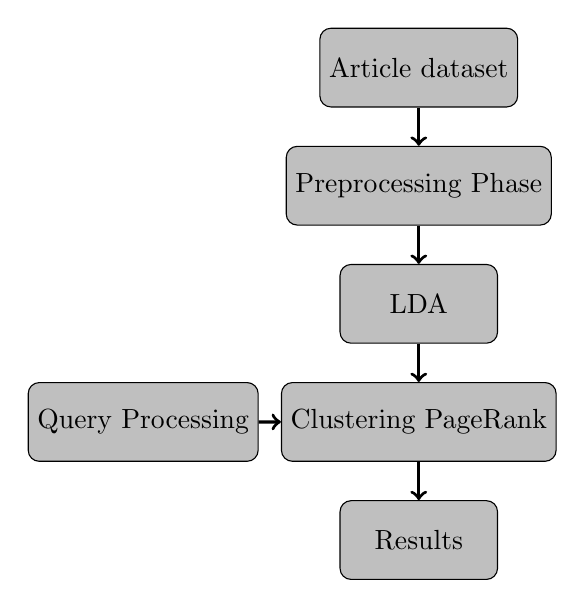
\begin{tikzpicture}[node distance=1.5cm]
    %\draw[step=1cm,gray,very thin] (-8,-8) grid (8,8);
	\node (Dataset) [process] {Article dataset};
	\node (Cleaning)[process, below of=Dataset] {Preprocessing Phase};
	\node (Training) [process, below of=Cleaning] {LDA};
	\node (Cluster PR) [process, below of=Training] {Clustering PageRank};
	\node (Query) at (-3.5, -4.5) [process] {Query Processing};
	\node (Result) [process, below of=Cluster PR] {Results};
	\draw [->, very thick] (Dataset) edge (Cleaning); 
	\draw [->, very thick] (Cleaning) edge (Training);
	\draw [->, very thick] (Training) edge (Cluster PR);
	\draw [->, very thick] (Cluster PR) edge (Result);
	\draw [->, very thick] (Query) edge (Cluster PR);
\end{tikzpicture}
	\caption{Pipeline}
    \label{fig:pipeline}
\end{figure}
